\chapter{Introduction}


\section{Design philosophy}

RASPA3 is a molecular simulation code for computing adsorption and diffusion in nanoporous materials, 
and thermodynamic and transport properties of fluids. 
It implements force field based classical Monte Carlo/Molecular Dynamics in various ensembles.
RASPA3 can be used for the simulation of molecules in gases, fluids, zeolites, aluminosilicates,
metal-organic frameworks, and carbon nanotubes.
One of the main applications of RASPA3 is to compute adsorption isotherms and to 
understand the atomic-level mechanism of adsorption and separations.


RASPA3 is redesigned and rewritten from the ground up in C++23, based on the following ideas:
\begin{itemize}
  \item{Composition and value semantics}\\
  Major improvements in efficiency result from the implementation of C++ code based on composition 
  and value semantics (in contrast to inheritance and reference semantics). Composition is a structural 
  approach in which complex objects are built from simple building blocks. Value semantics avoid 
  sharing mutable state and upholds the independence of values to support local reasoning. 
  References are only used implicitly,  at function boundaries, and are never stored. 
  This style of coding has many advantages. Avoiding complex inheritance hierarchies and reducing the 
  need for virtual functions lead to major code simplifications. It encourages code clarity and 
  local reasoning. With composition, components are directly included in an object, removing the 
  necessity for pointers, manual memory allocations, and indirections. This leads to straightforward 
  memory patterns and access safety. Lifetimes of objects are coupled with composition, eliminating the 
  need for explicit memory management. These lead to better compiler optimization and therefore performance of the code.
  \item{Correctness and accuracy}\\
  For all the techniques and algorithms available in RASPA3 we have implemented the 'best' ones available in literature. 
  For example, RASPA3 uses Configurational-Bias Monte-Carlo, it uses the Ewald summation for electrostatics,
  molecular dynamics is based on 'symplectic' integrators, all Monte-Carlo moves obey detailed balance etc.
  Unit tests test the smallest functional units of code and prevent developers breaking existing code when 
  refactoring or adding new code.
  The unit tests in RASPA3 are arranged hierarchically. Atoms are placed at several distances and the 
  Lennard-Jones potentials are tested and compared with the analytically computed energy. 
  Then molecules are placed within a zeolite framework at predetermined positions and compared to the 
  energies computed with RASPA2.
  The various energy routines used in biased-sampling are tested by comparing to the general routines.
  The various routines for the gradients are tested by comparing the computed gradients to the values 
  computed by finite difference schemes based on the energy. Likewise, the strain-derivative tensor 
  (related to the pressure) is tested by comparing to the values computed by finite difference schemes 
  based on the energy of a strained cell.
  \item{Input made easy}\\
  The input of RASPA3 has been changed to JSON format. 
  JSON stands for JavaScript Object Notation. It is a lightweight data-interchange format in plain text 
  written in JavaScript object notation. It is language independent.
  The requirements for the input files is kept as minimal as possible. 
  Only for more advanced options extra commands in the input file are
  needed. Also the format of the input is straightforward. Default settings are usually the best ones. 
  Fugacity coefficients and excess adsorption are automatically computed.
  \item{Output made easy}\\
  Similarly, the JSON format is now also used for the output. Where previously all initial data 
  (e.g. hardware info, unit conversion factors) and statistics (e.g. CPU timings, MC move statistics) 
  were written to a text file, these are now written as a nested dictionary to a JSON file.
  \item{Integrated simulation environment}\\
  The RASPA3 C++ simulation engine is made available to Python via a Pybind11 interface. 
  For use in Python, RASPA3 is built as a shared library, allowing its functions to be used by Python 
  users and enabling seamless interactions with the simulation routines.
  Through the API, the library allows for invocation of RASPA3's simulation routines from Python scripts, 
  calling the same simulation routines as via the JSON input. This execution directly from Python enables 
  the ability to prototype simulation settings and incorporate RASPA3 into existing workflows.
  Extension and modification of the code is relatively straightforward.
\end{itemize}

\section{Units and conventions}
\begin{itemize}
\item{The standard units in RASPA from which all other units are derived are:}\\
\vskip 0.1cm
\begin{tabularx}{\linewidth}{l|l|l|l}
 quantity & symbol & unit & value\\
\hline
 length      & $l$    & \AA ngstrom   & $10^{-10}$ m\\
 temperature & $T$    & Kelvin        & K\\
 mass        & $m$    & atomic mass   & $1.6605402\times 10^{-27}$ kg\\
 time        & $t$    & pico seconds  & $10^{-12}$ s\\
 charge      & $q$    & atomic charge & $1.60217733\times 10^{-19}$ C/particle\\
\hline
\end{tabularx}
\vskip 0.1cm

\noindent Some examples of derived units:\\

\begin{tabularx}{\linewidth}{l|l|l|l}
 quantity & symbol & units & conversion value\\
\hline
 energy             & $U$    & $J=\text{mass}\times\text{length}^2/\text{time}^2$ & $1.66054\times10^{-23}$ (=10 J/mol)\\
 pressure           & $p$    & $\text{Pa}=\text{mass}/(\text{length}\times\text{time}^2)$  & $1.66054\times10^7$\\
 diffusion constant & $D$    & $D=\text{length}^2/\text{time}$ & $1\times10^{-8}$\\
 force              & $f$    & $f=\text{length}/\text{time}^2$ & $1.66054\times 10^{-13}$\\
 \dots              & \dots  & \dots                                & \dots \\
\hline
\end{tabularx}\\

A pressure input of 10 Pascal in the input file, is converted to 'internal units' by dividing by $1.66054\times10^7$. In the
output any internal pressure is printed, multiplied by $1.66054\times10^7$. It is not necessary to convert units besides
input and output, with a few exceptions. One of them is the Coulombic conversion factor
\begin{equation}
  \frac{q_i q_j}{4\pi \epsilon_0}=\frac{\text{charge}^2}{4 \pi \times \text{electric constant}\times\text{length}\times\text{energy}}=138935.4834964017
\end{equation}
with the electric constant as $8.8541878176\times10^{-12}$ in units of $\text{C}^2/(\text{N}.\text{m}^2)$. This factor is needed to convert the
electrostatic energy to the internal units at every evaluation. 

\noindent
The Boltzmann's constant $k_B$ is
\begin{equation}
 k_B=\text{Boltzmann constant}/\text{energy}=0.8314464919
\end{equation}
with the Boltzmann constant as $1.380650324\times10^{-23}$ in units of J/K, and $k_B=0.8314464919$ in internal units.

\item{Numbering is based on the C-convention, i.e. starting from zero.}
\item{Files in the current directory always have preference.}\\
Sometimes one would like to try various parameters for force field fitting for example. In order to avoid
making a lot of directories for each force field it is more convenient to have the 
'pseudo\_atoms.def', 'force\_field\_mixing\_rule.def'
and 'force\_field.def' files in the \emph{current} directory.
\end{itemize}

\section{Compiling and installing RASPA}

\subsection{Requirements}

CMake 3.28 and later support C++ modules. 
C++20 named modules are now supported by the Ninja Generator 1.11 or newer in combination 
with the LLVM/Clang 16.0 and newer, MSVC toolset 14.34 and newer, or GCC 14 and newer. 
We recommend LLVM/Clang 18 or higher for compiling RASPA3. This version has support 
for \verb+std::format+, \verb+std::print+, and \verb+std::jthread+. 
The output-files of RASPA3 are in UTF-8 encoding and contain unicode characters (e.g. for \AA).
RASPA3 depends on
\begin{itemize}
\item{C++23 compliant compiler}
\item{Cmake 3.28}
\item{Ninja Generator 1.11}
\item{Openmp}
\item{hdf5}
\item{lapack and blas (64-bit integers)}
\item{pybind11}
\end{itemize}

\subsection{RASPA from 'git'}

Working with 'git' and a remote repository  means that you will have to distinguish between two locations of the code:
\begin{enumerate}
 \item{The repository (visible to everyone)}
 \item{your local copy (only visible to you)}
\end{enumerate}

To check-out the code for the first time do:
\begin{verbatim}
     git clone https://github.com/iraspa/RASPA3
\end{verbatim}
After that, you can update the code by using
\begin{verbatim}
     git pull
\end{verbatim}

\subsection{Installing RASPA}

Download one of the precompiled packages from
\begin{framed}
  \begin{quote}
    \url{https://github.com/iRASPA/RASPA3/releases}
  \end{quote}
\end{framed}
In Figure \ref{fig: binary_packages} one can find the list of packages. 
These include packages for macOS (both intel and apple silicon), and many linux distributions

\begin{figure}[p]
 \centering
  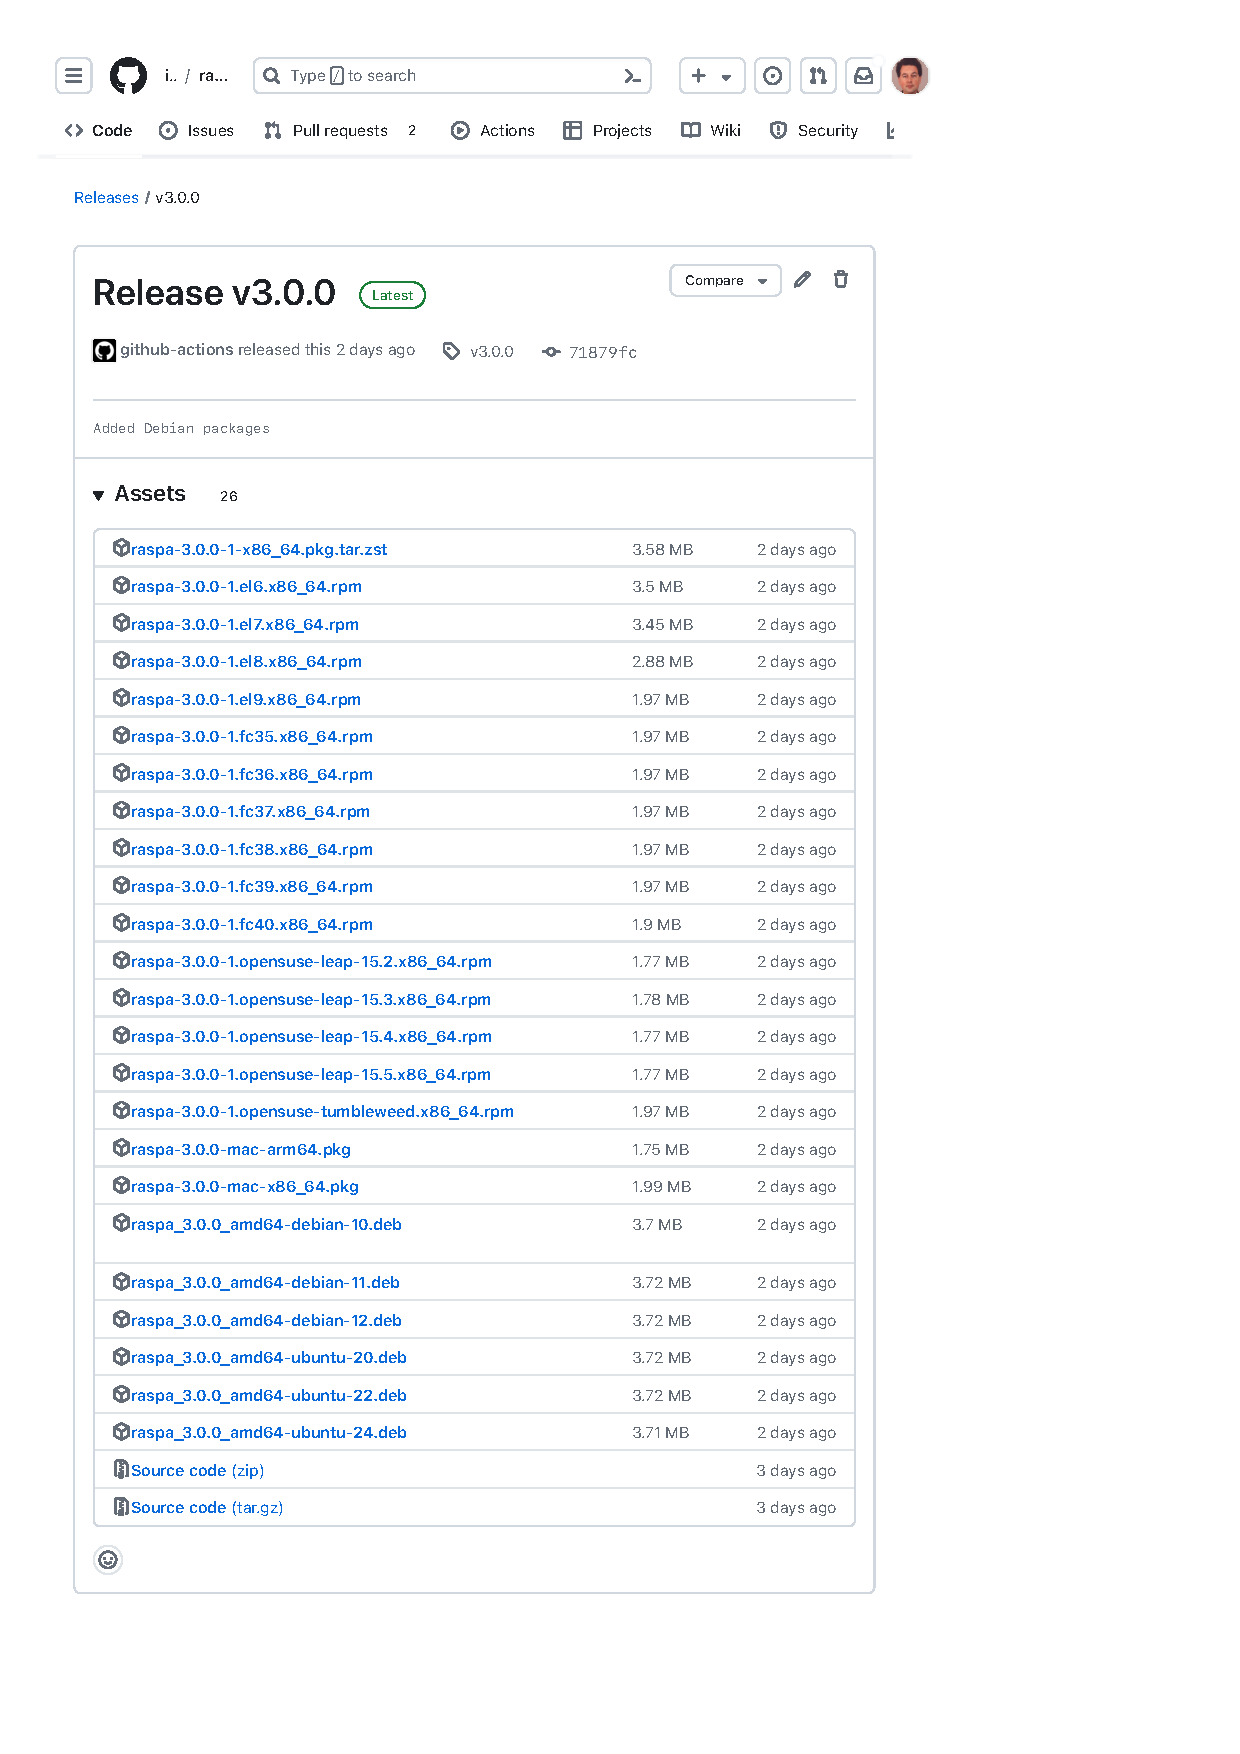
\includegraphics[width=0.85\linewidth]{introduction/figure_binary_packages.pdf}
  \caption{List of available binary packages: Linux distributions based on Red Hat and OpenSUSE (rpm-packages), Debian (deb-packages), and Arch Linux (tar.zst packages), and installers for intel- and apple-silicon macs.}
  \label{fig: binary_packages}
\end{figure}

\subsection{Compiling RASPA}

Using \verb+cmake --list-presets+ you can see the list of CMake presets.
These include
\begin{itemize}
  \item{"macos-intel"}
  \item{"macos-intel-debug"}
  \item{"macos-apple-silicon"}
  \item{"macos-apple-silicon-debug"}
  \item{"linux"}
  \item{"linux-opensuse-leap-15.2"}
  \item{"linux-opensuse-leap-15.3"}
  \item{"linux-opensuse-leap-15.4"}
  \item{"linux-opensuse-leap-15.5"}
  \item{"linux-opensuse-tumbleweed"}
  \item{"linux-archlinux"}
  \item{"linux-redhat-6"}
  \item{"linux-redhat-7"}
  \item{"linux-redhat-8"}
  \item{"linux-redhat-9"}
  \item{"linux-debian-12"}
  \item{"linux-debian-11"}
  \item{"linux-debian-10"}
  \item{"linux-ubuntu-24"}
  \item{"linux-ubuntu-22"}
  \item{"linux-ubuntu-20"}
  \item{"linux-fedora-35"}
  \item{"linux-fedora-36"}
  \item{"linux-fedora-37"}
  \item{"linux-fedora-38"}
  \item{"linux-fedora-39"}
  \item{"linux-fedora-40"}
\end{itemize}

\noindent
Installation on macOS is then accomplished for example by
\begin{framed}
\begin{verbatim}
cmake -B build --preset macos-intel
ninja -C build install
\end{verbatim}
\end{framed}
or on linux
\begin{framed}
\begin{verbatim}
cmake -B build --preset linux-ubuntu-22
ninja -C build install
\end{verbatim}
\end{framed}
afterwhich the unit tests can be run
\begin{framed}
\begin{verbatim}
ctest --test-dir build/tests --verbose
\end{verbatim}
\end{framed}

\noindent
Packages can be created with
\begin{framed}
\begin{verbatim}
ninja -C build package
\end{verbatim}
\end{framed}

\noindent
Doxygen code documentation can be created with
\begin{framed}
\begin{verbatim}
ninja -C build documentation
\end{verbatim}
\end{framed}

\paragraph{Installing required packages on Ubuntu-24 or higher}

\begin{verbatim}
apt-get install -y git ca-certificates cmake ninja-build
apt-get install -y llvm lld clang clang-tools clang-tidy
apt-get install -y libc++-dev libc++abi-dev libomp-dev libclang-rt-dev
apt-get install -y python3 pybind11-dev python3-pybind11 python3-dev
apt-get install -y liblapack64-dev libblas64-dev
apt-get install -y libhdf5-cpp-103-1t64 libhdf5-dev python3-h5py python3-tables
\end{verbatim}

\paragraph{Installing required packages on Fedora-40 or higher}

\begin{verbatim}
dnf install -y wget git rpm-build
dnf install -y llvm lld cmake clang clang-tools-extra ninja-build
dnf install -y libcxx libcxxabi libcxx-devel libcxxabi-devel 
dnf install -y libomp-devel libcxx-static libcxxabi-static
dnf install -y lapack-devel lapack64 blas64
dnf install -y python3 python3-devel python3-pybind11
dnf install -y pybind11-devel
dnf install -y hdf5 hdf5-devel hdf5-static python3-h5py python3-tables
\end{verbatim}

\paragraph{Installing required packages on macOS using Homebrew}

\begin{verbatim}
dnf install -y wget git rpm-build
dnf install -y llvm lld cmake clang clang-tools-extra ninja-build
dnf install -y libcxx libcxxabi libcxx-devel libcxxabi-devel
dnf install -y libomp-devel libcxx-static libcxxabi-static
dnf install -y lapack-devel lapack64 blas64
dnf install -y python3 python3-devel python3-pybind11
dnf install -y pybind11-devel hdf5
\end{verbatim}

\subsection{Running RASPA\label{Introduction: running RASPA}}
Running RASPA is based on two files:
\begin{itemize}
 \item{A 'run' file to execute the program}\\
  an example file is:
\begin{verbatim}
#! /bin/sh -f
export RASPA_DIR=/usr/
${RASPA_DIR}/bin/raspa3
\end{verbatim}
  This type of file is know as a 'shell script'. RASPA needs the variable 'RASPA\_DIR' to be set in order
  to look up the molecules, frameworks, etc. The scripts sets the variable and runs RASPA. RASPA can then be run
  from any directory you would like.
 \item{An 'input'-file describing the type of simulation and the parameters}\\
  In the same directory as the 'run'-file, there needs to be a file called \verb+simulation.json+. An example file is:
\begin{verbatim}
{
  "SimulationType" : "MonteCarlo",
  "NumberOfCycles" : 100000,
  "NumberOfInitializationCycles" : 1000,
  "NumberOfEquilibrationCycles" : 10000,
  "PrintEvery" : 1000,

  "Systems" :
  [
    {
      "Type" : "Box",
      "BoxLengths" : [30.0, 30.0, 30.0],
      "ExternalTemperature" : 300.0,
      "ChargeMethod" : "None",
      "OutputPDBMovie" : true,
      "SampleMovieEvery" : 10
    }
  ],

  "Components" :
  [
    {
      "Name" : "methane",
      "MoleculeDefinition" : "ExampleDefinitions",
      "TranslationProbability" : 1.0,
      "CreateNumberOfMolecules" : 100
    }
  ]
}
\end{verbatim}
  This tells RASPA to run a Monte-Carlo simulation of 100 methane molecules in a $30\times30\times30$ \AA\ cubic box (with 90$^\circ$ angles)
  at 300 Kelvin. It will start with 1000 cycles to initialize the system,
    10000 cycles to equilibrate the system, and will use 100000 cycle to obtain thermodynamic properties
  of interest. Every 1000 cycles a status-report is printed to the output. The Monte-Carlo program will use only the 'translation move'
  where a particle is given a random translation and the move is accepted or rejected based on the energy difference.
  \end{itemize}


In order to run it on a cluster using a queuing system one needs an additional file 'bsub.job' (arbitrary name)
\begin{itemize}
 \item{'gridengine'}
  \begin{verbatim}
     #!/bin/bash
     # Serial sample script for Grid Engine
     # Replace items enclosed by {}
     #$ -S /bin/bash
     #$ -N Test
     #$ -V
     #$ -cwd
     echo $PBS_JOBID > jobid
     exprot RASPA_DIR=/usr
     $RASPA_DIR/bin/raspa3
  \end{verbatim}
The job can be submitted using 'qsub bsub.job'.
 \item{'torque'}
  \begin{verbatim}
     #!/bin/bash
     #PBS -N Test
     #PBS -o pbs.out
     #PBS -e pbs.err
     #PBS -r n
     #PBS -V
     #PBS -mba
     cd $PBS_O_WORKDIR
     echo $PBS_JOBID > jobid
     export RASPA_DIR=/usr
     ${RASPA_DIR}/bin/raspa3
  \end{verbatim}
The job can be submitted using 'qsub bsub.job'.
 \item{'slurm'}
\begin{verbatim}
  #!/bin/bash 
  #SBATCH -N 1
  #SBATCH --job-name=Test
  #SBATCH --export=ALL
  echo $SLURM_JOBID > jobid
  valhost=$SLURM_JOB_NODELIST
  echo $valhost > hostname
  module load slurm
  export RASPA_DIR=/usr
  ${RASPA_DIR}/bin/raspa3
\end{verbatim}
The job can be submitted using 'sbatch bsub.job'.
\end{itemize}


\section{Output from RASPA}
RASPA generates output from the simulation. Some data is just information on the status, while other data are written because you
specifically asked the program to compute it for you. The output is written to be used with other programs like:
\begin{itemize}
 \item{gnuplot}
 \item{iRASPA}
 \item{VMD}
\end{itemize}

\section{Citing RASPA}

If you are using RASPA and would like to cite it in your journal articles or book-chapters, then for RASPA:

\begin{quote}
Y.A. Ran, S. Sharma, S.R.G. Balestra, Z. Li, S. Calero, T.J.H Vlugt, R.Q. Snurr, and D. Dubbeldam
\newblock RASPA3: A Monte Carlo Code for Computing Adsorption and Diffusion in Nanoporous Materials and Thermodynamics Properties of Fluids
\newblock {\em J. Chem. Phys.}, 2024.
\end{quote}
\begin{quote}
D. Dubbeldam, S. Calero, D.E. Ellis, and R.Q. Snurr,
\newblock RASPA: Molecular Simulation Software for Adsorption and Diffusion in Flexible Nanoporous Materials,
\newblock {\em Mol. Simulat.}, \url{http://dx.doi.org/10.1080/08927022.2015.1010082}, 2015.
\end{quote}
For the inner workings of Monte Carlo codes:
\begin{quote}
D. Dubbeldam, A. Torres-Knoop, and K.S. Walton,
\newblock On the Inner Workings of Monte Carlo Codes,
\newblock  \url{http://dx.doi.org/10.1080/08927022.2013.819102}
\newblock {\em Mol. Simulat.}, 39(14-15), 1253-1292, 2013.
\end{quote}
For the description of Molecular Dynamics and diffusion:
\begin{quote}
D. Dubbeldam and R.Q. Snurr,
\newblock Recent Developments in the Molecular Modeling of Diffusion in Nanoporous Materials,
\newblock  \url{http://dx.doi.org/10.1080/08927020601156418},
\newblock {\em Mol. Simulat.}, 33(4-5), 305-325, 2007.
\end{quote}
For the description of the implementation of force fields:
\begin{quote}
D. Dubbeldam, K.S. Walton, T.J.H. Vlugt, and S. Calero,
\newblock Design, Parameterization, and Implementation of Atomic Force Fields for Adsorption in Nanoporous Materials,
\newblock  \url{https://doi.org/10.1002/adts.201900135},
\newblock {\em Adv. Theory Simulat.}, 2(11), 1900135, 2019.
\end{quote}

